\documentclass{article}

\usepackage{qa}

\begin{document}
\customtitle{Homework 1}
\customauthor{Hamza Kamal}
\customdate{\today}
\qna{
     (2pts) Register Transfer Language (RTL) \\
     Trace the data flow of the following code using RTL. Include the first instruction fetch. LDR R2, [R1]
} {
     \begin{math}
          MAR \leftarrow PC \\
          PC \leftarrow PC + 2 \\
          IR \leftarrow mem[MAR] \\
          MAR \leftarrow R1 \\
          R2 \leftarrow mem[MAR]
     \end{math}
}

\qna{
     (2 pts) Application Program Status Register (APSR)’s flags \\
     After the following piece of instructions is executed, what value will be maintained in each of NZCV flags in APSR?
} {
     \begin{center}
          \begin{tabular}{|c c|}
               \hline
               Flag & Value \\
               \hline
               N & 1 \\
               \hline
               Z & 0 \\
               \hline
               C & 0 \\
               \hline
               V & 1 \\
               \hline
          \end{tabular}
     \end{center}
}

\qna{
     (4 pts) Memory Endianness and Alignment \\
     1. As you see the following example with \#1234 at memory address 0x20000000, allocate \#1234567890 to memory address 0x20001000. (2pts) \\
     \underline{An example:} \\
     Big Endian: \\
     \linebreak
     \begin{tabular}{|c c|}
          \hline
          Address & Data Contents (in hex) \\
          \hline
          0x20000000 & 04 \\
          \hline
          0x20000001 & D2 \\
          \hline
          0x20000002 & \\
          \hline
          0x20000003 & \\
          \hline
     \end{tabular} \\
     \linebreak
     Little Endian: \\
     \linebreak
     \begin{tabular}{|c c|}
          \hline
          Address & Data Contents (in hex) \\
          \hline
          0x20000000 & D2 \\
          \hline
          0x20000001 & 04 \\
          \hline
          0x20000002 & \\
          \hline
          0x20000003 & \\
          \hline
     \end{tabular}
     \linebreak
} {
     $\#1234567890$ \\
     $\#1234567890 \text{ in hex} = 0x499602D2_{16}$ \\
     Big Endian: \\
     \linebreak
     \begin{tabular}{|c c|}
          \hline
          Address & Data Contents (in hex) \\
          \hline
          0x20000000 & 49 \\
          \hline
          0x20000001 & 96 \\
          \hline
          0x20000002 & 02 \\
          \hline
          0x20000003 & D2 \\
          \hline
     \end{tabular} \\
     \linebreak
     Little Endian: \\
     \linebreak
     \begin{tabular}{|c c|}
          \hline
          Address & Data Contents (in hex) \\
          \hline
          0x20000000 & D2 \\
          \hline
          0x20000001 & 02 \\
          \hline
          0x20000002 & 96 \\
          \hline
          0x20000003 & 49 \\
          \hline
     \end{tabular}
     \linebreak
}

\qna{
     As you see the following example with exampleData, allocate myData to the memory and fill out the spaces to indicate how each data element is mapped. Assume that the memory is based on a 32-bit addressing system. (2pts) \\
     \underline{An Example: } \\
     \texttt{struct exampleData \{ \\
               \indent char a; \\
               \indent short b; \\
     \}} \\
     \linebreak
     \begin{tabular}{|c|c|c|c|c|}
          \hline
          & + 0th & + 1st & + 2nd & + 3rd \\
          \hline
          0th byte & a &  & b & b \\
          \hline
          4th byte &  &  &  &  \\
          \hline
          8th byte &  &  &  &  \\
          \hline
     \end{tabular}
     \linebreak
} {
     \texttt{struct myData \{ \\
          \indent char a; \\
          \indent long long int b; \\
          \indent double c; \\
          \indent short d; \\
          \indent char *e; \\
          \indent float f; \\
     \}} \\
     \linebreak
     \begin{tabular}{|c|c|c|c|c|}
          \hline
           & + 0th & + 1st & + 2nd & + 3rd \\
          \hline
          0th byte & a &  & b & b \\
          \hline
          4th byte & b & b & b & b \\
          \hline
          8th byte & b & b &  & c \\
          \hline
          12th byte & c & c & c & c \\
          \hline
          16th byte & c & c & c &  \\
          \hline
          20th byte & d & d &  & e \\
          \hline
          24th byte &  & f & f & f \\
          \hline
          28th byte & f &  &  &  \\
          \hline
          32nd byte &  &  &  &  \\
          \hline
     \end{tabular}
     \linebreak
}

\qna {
     (4pts) Assemble the codes Using the following picture of Thumb2’s encoding formats, convert the following three assembly language instructions to the machine codes in hexadecimal. You have to show your work, otherwise you get zero. \\
     \begin{figure}[H]
          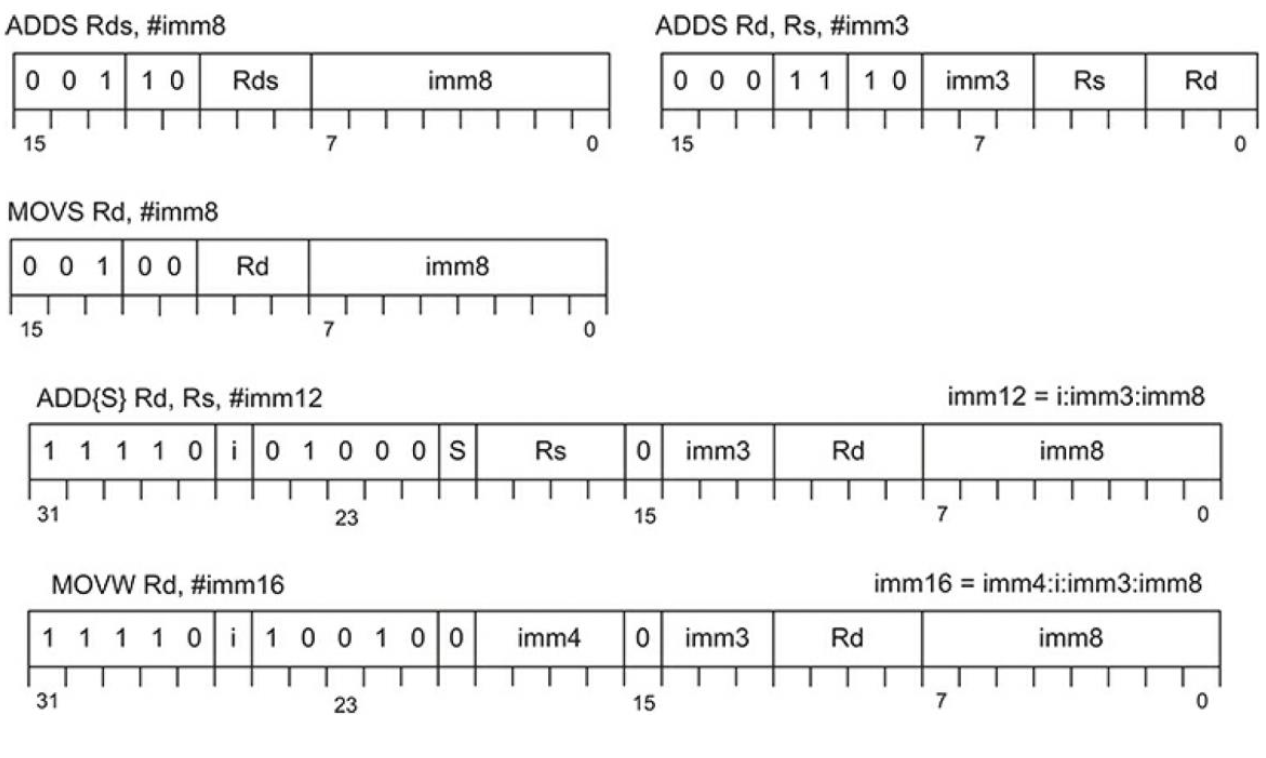
\includegraphics[width=\textwidth]{./img/machine_code.png}
     \end{figure}
     1. ADDS R7, R5, \#7 (2pts)
} {
     \begin{math}
          R5 = 101 \\
          R7 = 111 \\
          7 = 111_{2}
     \end{math} \\
     \begin{tabular}{|c|c|c|c|c|c|}
          \hline
          000 & 11 & 10 & \text{imm3} & \text{Rs} & \text{Rd} \\
          \hline
     \end{tabular} \\
     \begin{tabular}{|c|c|c|c|c|c|}
          \hline
          000 & 11 & 10 & 111 & 101 & 111 \\
          \hline
     \end{tabular}
}

\qna{
     2. MOVW R10, \#0x1234. (2pts)
} {
     \begin{math}
          R10 = 1010 \\
          0x1234 = 0001 0010 0011 0100 \\
     \end{math} \\
     \begin{tabular}{|c|c|c|c|c|c|c|c|c|}
          \hline
          1111 & i & 10010 & 0 & \text{imm4} & 0 & \text{imm3} & \text{Rd} & \text{imm8} \\
          \hline
     \end{tabular} \\
     \begin{tabular}{|c|c|c|c|c|c|c|c|c|}
          \hline
          1111 & 0 & 10010 & 0 & 0010 & 0 & 010 & 1010 & 0011 0100 \\
          \hline
     \end{tabular}
}
\end{document}